\subsection{Podnošenje prijave za auto školu}

Na slici  \ref{fig:ui_registracija} je prikazana stranica za prijavljivanje kandidata u auto školu. 
Informacije koje korisnik unosi su: ime, prezime, JMBG, telefon, email adresa i dodaje svoju sliku. 
Neophodno je da sve informacije budu unete, kao i da budu u ispravnom formatu, gde se poruka prikazuje ukoliko ne zadovoljavaju traženi format.

\begin{figure}[H]
  \begin{center}
      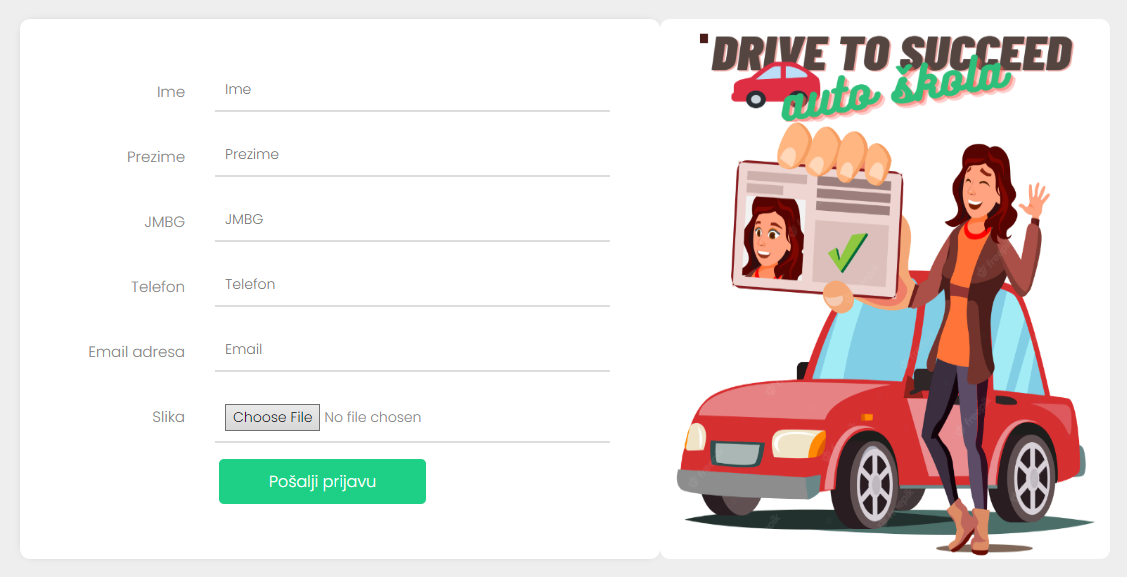
\includegraphics[width=140mm, height=70mm]{UI/UI_registracija.png}
  \end{center}
  \caption {Podnošenje prijave za auto školu}
  \label{fig:ui_registracija}

\end{figure}

\subsection{Prijavljivanje kandidata na nalog}

Slika \ref{fig:ui_registracija} prikazuje izgled stranice za prijavljivanje kanidata na svoj nalog. 
Kandidat unosi ID i loziknku koju je dobio na mejl. Takođe, kandidat ima opciju "Zapamti" za čuvanje ID-ja i lozinke pri sledećem prijavljivanju.
Klikom na opciju "Zaboravljena lozinka", kandidatu se šalje na mejl nova lozinka za oporavak naloga. 

\begin{figure}[H]
  \begin{center}
      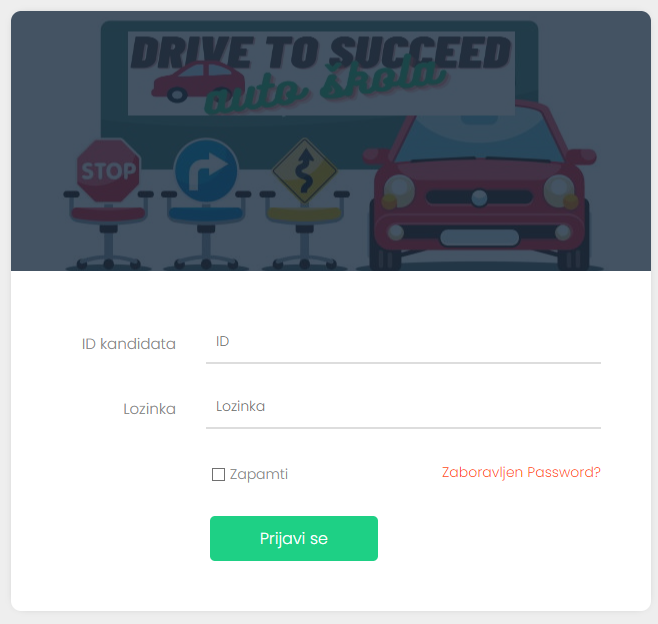
\includegraphics[width=140mm, height=80mm]{UI/UI_login.png}
  \end{center}
  \caption {Prijavljivanje kandidata na nalog}
  \label{fig:ui_login}

\end{figure}
